\section{SHA-1} \label{sec:SHA-1}

In cryptography, SHA-1 (Secure Hash Algorithm 1) is a cryptographic hash function which takes an input and produces a 160-bit (20 byte) hash value known as a message digest
\subsection{Algorithm overview}

In figure you can see one iteration within the SHA-1 compression function:
\begin{figure}[!h]
\centering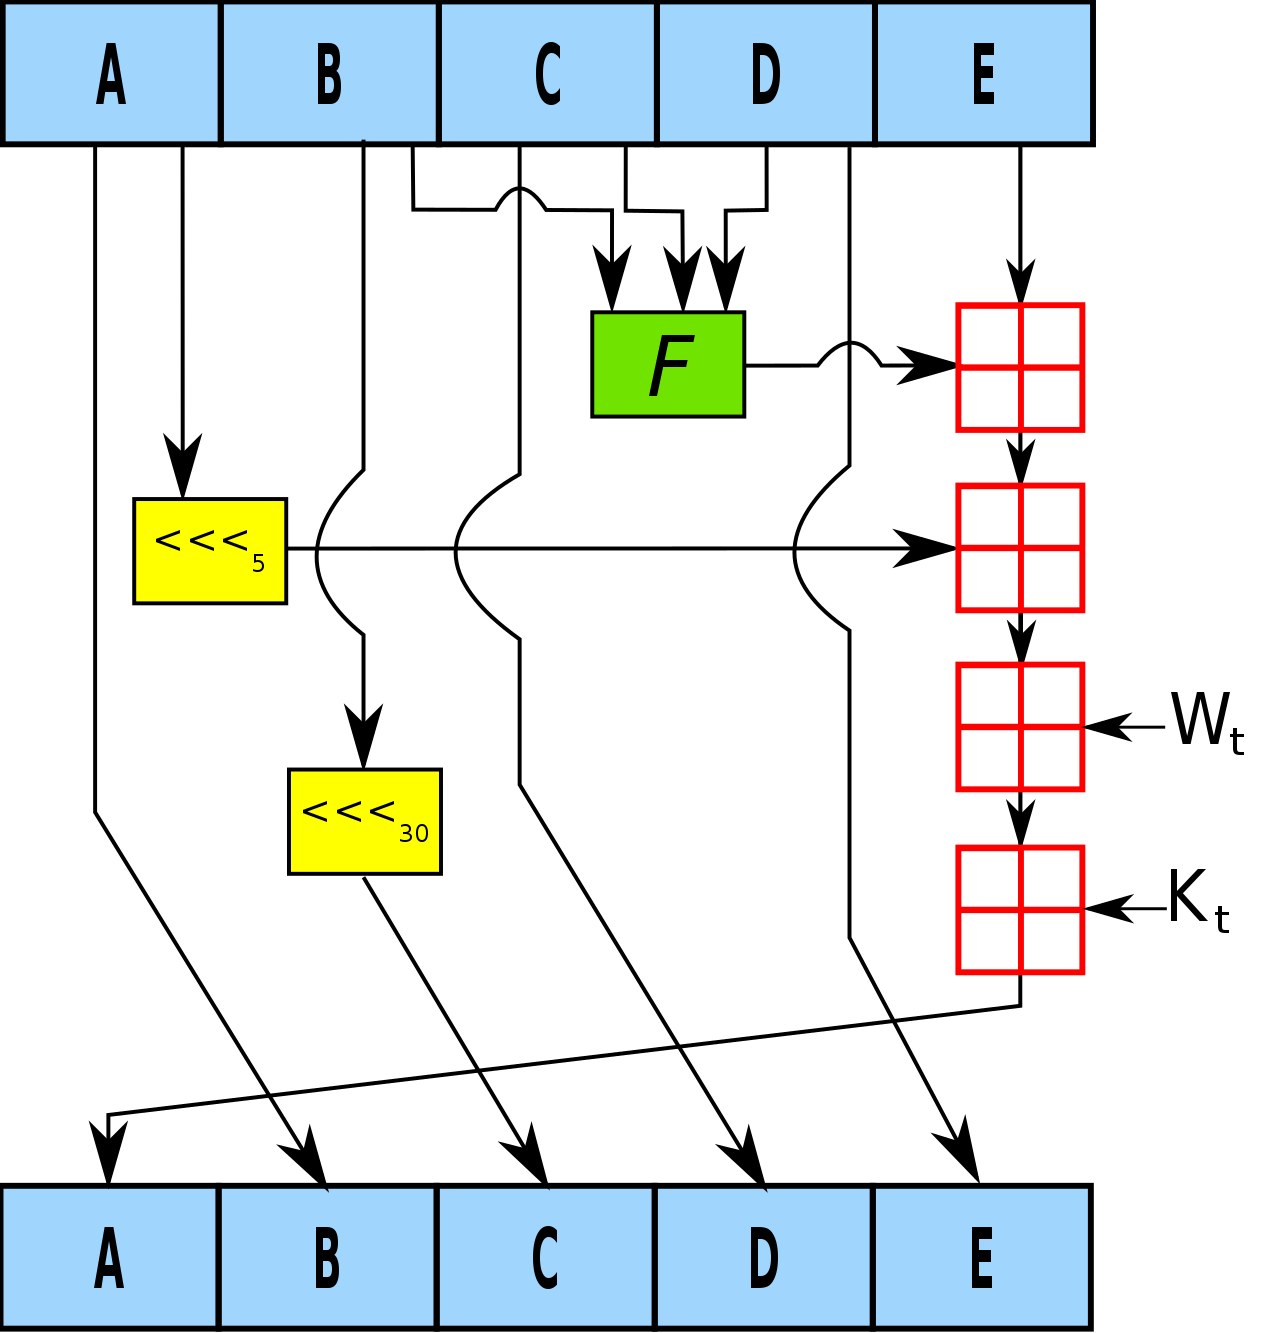
\includegraphics[scale=0.11]{SHA-1-wiki}
\caption{One iteration of SHA-1.
A, B, C, D and E are 32-bit words of the state; F is a nonlinear function that varies; $W_t$ is the expanded message word of round t; $K_t$ is the round constant of round t;}
\label{fig:SHA-1-wiki} 
\end{figure}
\footnote{You can find more details of the figure here \cite{sha-1-wiki}.}

\textit{Steps}\cite{sha-1-slideshare}:
\\
\begin{enumerate}
	\itemsep1em
	\item Padding of bits.
	\item Append length.
	\item Devide the input into 512-bit blocks.
		\begin{figure}[!h]
			\centering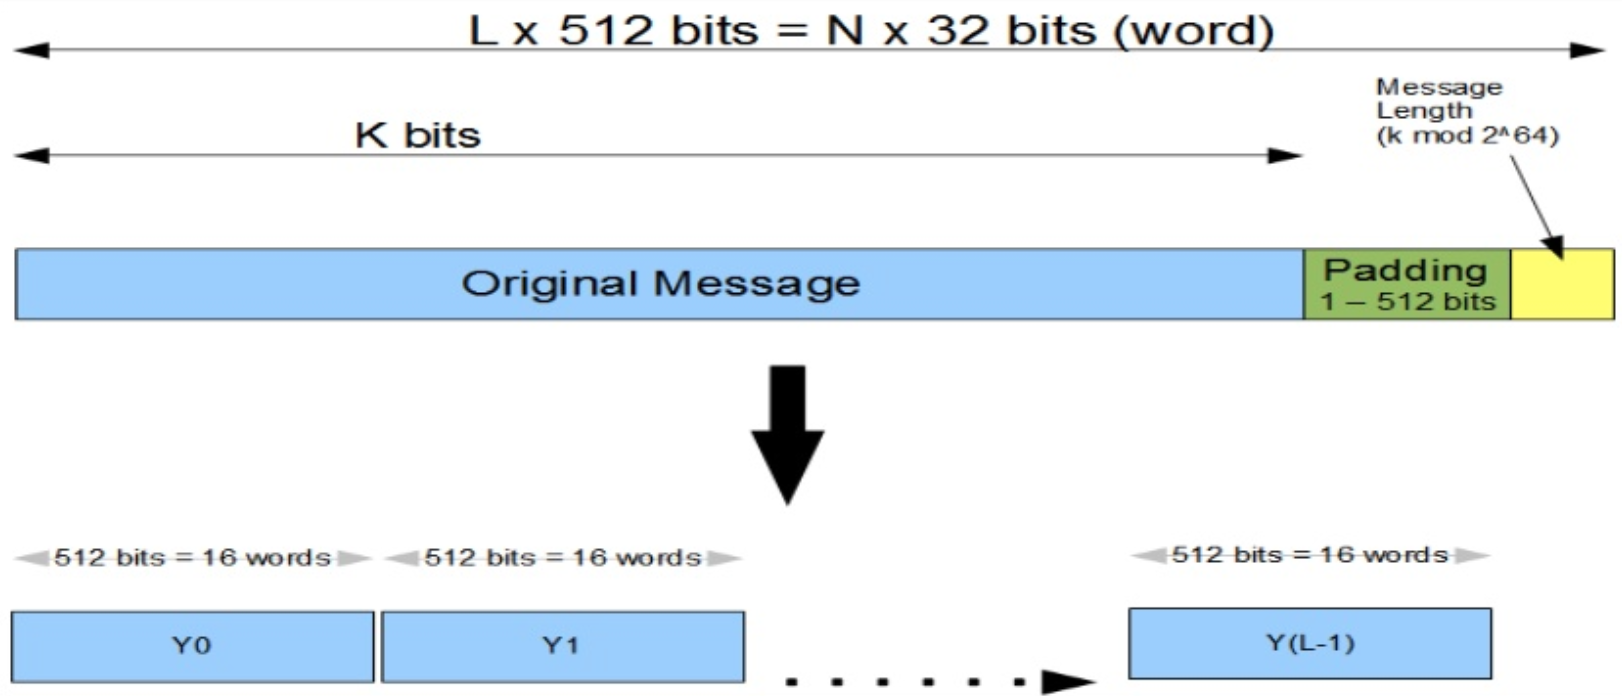
\includegraphics[scale=0.3]{SHA-1}
			\caption{Steps 1 to 3}
			\label{fig:SHA-1} 
		\end{figure}
	\item Initializing chaining variables
		\begin{figure}[!h]
			\centering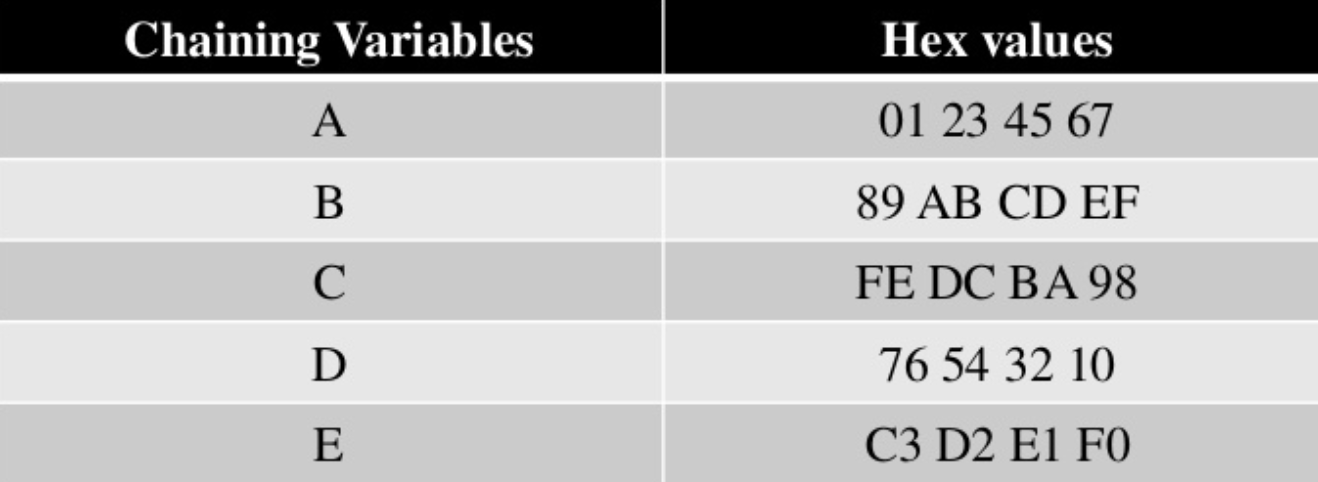
\includegraphics[scale=0.3]{SHA1-init}
			\caption{Steps 4}
			\label{fig:SHA-1-init} 
		\end{figure}
	\item Process blocks
		\begin{enumerate}[label=\alph*.]
			\item Copy chaining variables A-E into variables a-e.
			\item Divide current 512-bit block into 16 sub-blocks of 32-bit.
			\item SHA has 4 round, each consisting of 20 steps.\\
				Each round takes 3 inputs:\\
				512-bit block.\\
				The register abcde.\\
				A constant K[t] (where t = 0 to 79)
				\begin{figure}[!h]
					\centering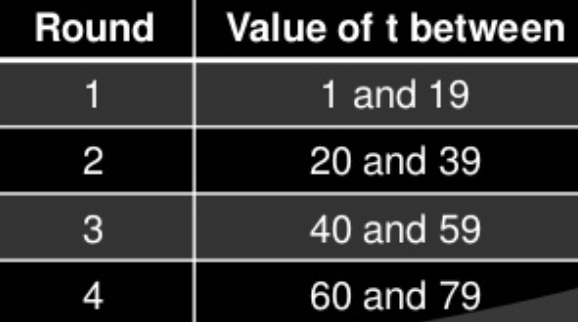
\includegraphics[scale=0.5]{SHA-1-k}
					\caption{Steps 4}
					\label{fig:SHA-1-k} 
				\end{figure}
				\item SHA has a total of 80 iterations (4 round X 20 iterations). Each iterations consist of the following operations:\\
				$abcde = (e + Process e + S^5(a) + W[t] + K[t])\ ||\ a\ ||\ S^{30}(b)\ ||\ c\ ||\ d$\\
					\begin{description}
						\item[abcde] The register made up of 5 variables a, b, c, d, e.
						\item[Process P:] A logical operation.\ref{fig:SHA-1-P} 
						\item[$S^t$] is a circular-shift of 32-bit sub-block by t bits.
						\item[W[t]] is a 32-bit derived from the current 32-bit sub-block.
						\item[K[t]] is one of the 5 additive constants.
					\end{description}
				\begin{figure}[!h]
					\centering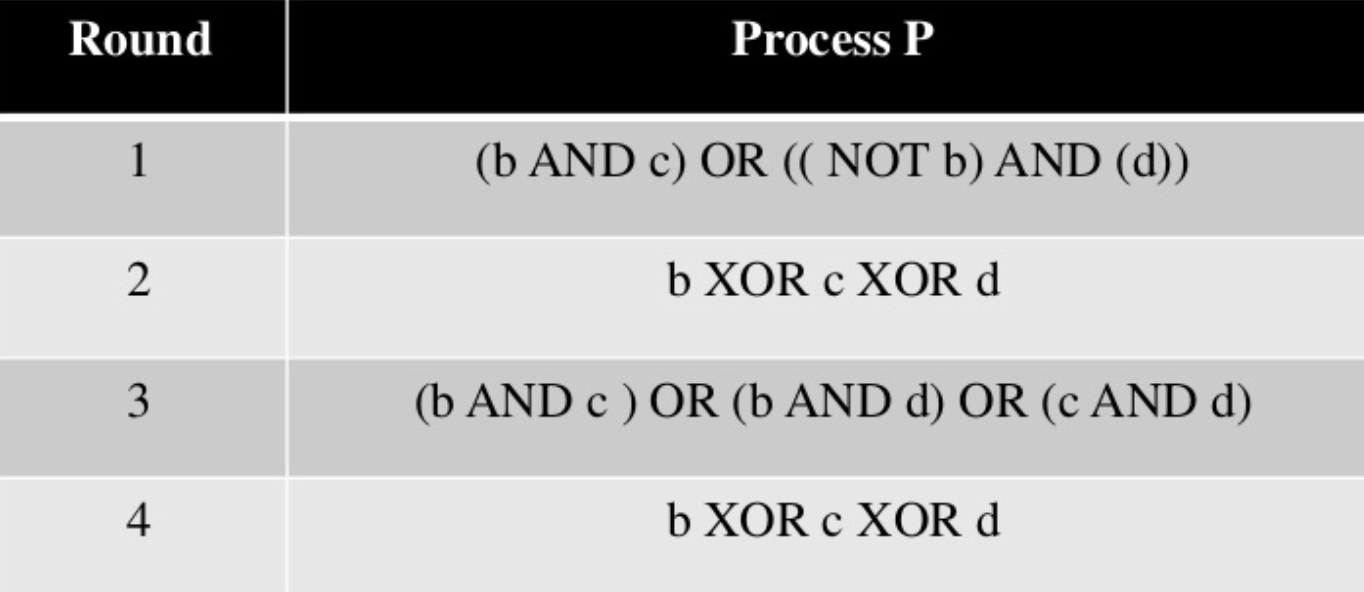
\includegraphics[scale=0.5]{SHA-1-P}
					\caption{Steps 4}
					\label{fig:SHA-1-P} 
				\end{figure}
					
		\end{enumerate}
\end{enumerate}

The values of W[t] are calculated as follows:
\begin{itemize}
	\item For the first 16 words of W (t = 0 to t = 15), the contents of the input message sub-block M[t] become the contents of W[t].
	\item For the remaining 64 values of W are derived using the equation:\\
	$W[t] = S^1(W[t-16] \oplus W[t-14] \oplus W[t-8] \oplus W[t-3]) $
\end{itemize}









